\documentclass[a4paper, 11pt, titlepage]{article}
\usepackage{graphicx}
\usepackage{pdfpages}
\usepackage{fancybox}
\usepackage[francais]{babel}
\usepackage[utf8]{inputenc}
% \usepackage[T1]{fontenc}
\usepackage{amsmath,amsfonts,amssymb}
\usepackage{fancyhdr}
\usepackage{stackrel}
\usepackage{babel,indentfirst}
\usepackage{xspace}
\usepackage{url}
\usepackage{titling}
\usepackage{listings}
\usepackage{color}
\usepackage{array}
\usepackage{hyperref}
\usepackage{makecell}
\usepackage{tikz}
\usepackage{float}
\usepackage{wrapfig}

%\setlength{\parindent}{0pt}
\setlength{\parskip}{1ex}
\setlength{\textwidth}{17cm}
\setlength{\textheight}{24cm}
\setlength{\oddsidemargin}{-.7cm}
\setlength{\evensidemargin}{-.7cm}
\setlength{\topmargin}{-.5in}


\lstset{
  sensitive=f,
  morestring=[d]",
  showstringspaces=false,
  basicstyle=\small\ttfamily,
  keywordstyle=\bf\small,
  commentstyle=\itshape,
  stringstyle=\sf,
  extendedchars=true,
  columns=[c]fixed
}



\predate{
\begin{center}
}
\postdate{
\\
\vspace{1.5cm}

\includegraphics[scale=0.7]{imag.png}
\end{center}}


\title {{ {\huge Documentation préliminaire du projet SMACK }} }

\author{\Large Equipe 5 \\
\\
    {\sc Ait El Kadi}~Ouiame
    {\sc Ansari}~Othmane
    {\sc Boudouin}~Philippe\\
    {\sc Boukrouh}~Insaf
    {\sc Giroux}~Baptiste
    {\sc Gouttefarde}~Léo\\
    {\sc Kodjo}~Edoh
    {\sc Nahyl}~Othmane
}

\date{Vendredi 25 Novembre 2016}

\lhead{Projet SMACK}
\rhead{Documentation}

\begin{document}
\pagestyle{fancy}
\maketitle

\setcounter{tocdepth}{2}

\tableofcontents
\newpage

\section {Les différents composants de la stack}

\subsection {Spark}

Apache Spark est un framework open source de traitements Big Data, construit pour effectuer des analyses sophistiquées et conçu pour la facilité d'utilisation et la rapidité. 
Spark permet une parallélisation massive avec une technologie in-memory. Les applications sur clusters Hadoop sont exécutées jusqu'à 100 fois plus vite en mémoire, 10 fois plus vite sur disque.

Il est écrit en Scala et s'exécute sur la machine virtuelle Java (JVM). Les langages supportés actuellement pour le développement d'applications sont : Scala, Java, Python, Clojure, R. Spark est complet et unifié pour répondre aux besoins de traitements de données (texte, graphe, etc.) en batch ou en flux temps-réel.


\subsubsection* {L'écosystème de Spark}

\begin{center}
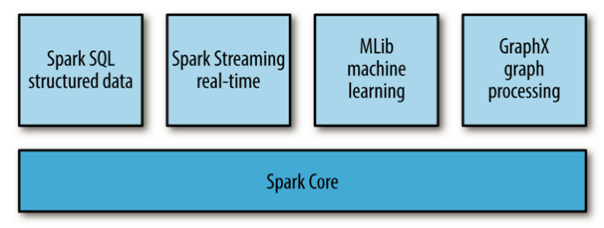
\includegraphics[scale=0.5]{res/eco_spark.png}
\end{center}


\begin{enumerate}

\item
\textbf{Spark Streaming} : Peut être utilisé pour traitement temps-réel des données en flux

\item
\textbf{Spark SQL} : Permet d'exécuter des requêtes de type SQL

\item
\textbf{Spark MLlib} : Librarie de machine learning qui contient tous les algorithmes et utilitaires d'apprentissage classiques (la classification, la régression, le clustering...)

\item
\textbf{Spark GraphX} : La nouvelle API pour les traitements de graphes et de parallélisation de graphes

\end{enumerate}

\subsubsection* {L'architecture de Spark}

\begin{center}
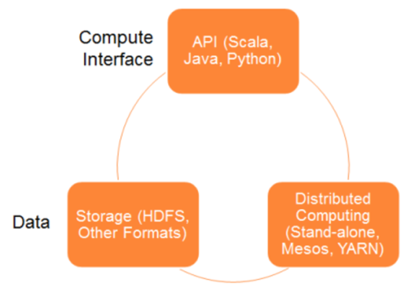
\includegraphics[scale=0.5]{res/archi_spark.png}
\end{center}


\begin{enumerate}

\item
\textbf{L'API}

L'API permet aux développeurs de créer des applications Spark en utilisant une API standard. L'API existe en Scala, Java et Python.

\item
\textbf{Le stockage des données}

Spark utilise le système de fichiers HDFS pour le stockage des données. Il peut fonctionner avec n'importe quelle source de données compatible avec Hadoop, dont HDFS, HBase, \textbf{Cassandra}, etc.


\item
\textbf{Le cluster manager}

Spark peut être déployé comme un serveur autonome ou sur un framework de traitements distribués comme \textbf{Mesos} ou YARN.

\end{enumerate}


\subsubsection* {Les RDDs}


Le concept clé de Spark est les RDDS. Un RDD (Resilient Distributed Dataset) est une abstraction de collection partitionnée d'enregistrements pouvant être distribuée entre machines de manière tolérante aux pannes. 


Les RDD supportent deux types d'opérations:

\begin{itemize}

\item
Les transformations : les transformations ne retournent pas de valeur seule, rien n'est évalué, elles retournent un nouveau RDD.

\item
Les actions : les actions évaluent et retournent une nouvelle valeur.

\end{itemize}



\subsubsection* {Le workflow}


Le workflow de Spark comporte quatre phases principales :

\begin{itemize}

\item
Les RDDs (transformations et actions) forment le DAG (Direct Acyclic Graph)

\item
Le DAG est divisé en ensembles de tâches qui sont ensuite soumises au gestionnaire de cluster

\item
Un ensemble de tâche combine les tâches qui ne nécessitent pas de shuffling/répartition

\item
Les tâches sont exécutées sur les workers qui ensuite retournent les résultats au client

\end{itemize}


\begin{center}
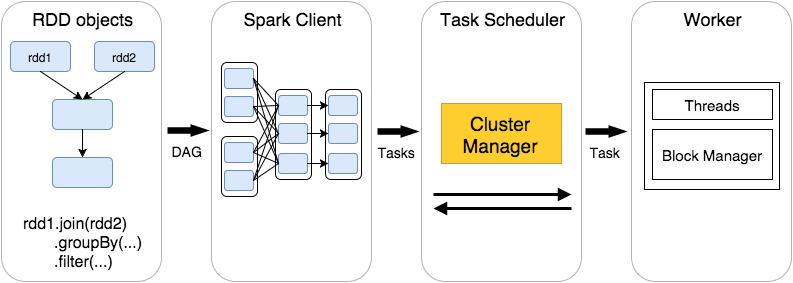
\includegraphics[scale=0.5]{res/workflow_spark.png}
\end{center}

\newpage
\subsection {Mesos}

Mesos est un gestionnaire de cluster basé sur l'architecture maître / esclave, qui permet d'abstraire les ressources des machines du cluster afin d'éliminer les problèmes de scalabilité.

Il permet aux datacenters de fonctionner comme s'ils étaient un unique serveur hébergeant plusieurs applications


Traditionnellement, les datacentres comportaient des clusters réservés pour un framework/application bien précise. Ceci impliquait des problèmes de scalabilité dès que des noeuds d'un cluster deviennent indisponibles. Mesos permet à plusieurs frameworks de cohabiter dans le même cluster.


Mesos se base sur un principe appellé Two-Tier Scheduling (Planification à deux niveaux):

\begin{itemize}

\item
De manière continue, les esclaves proposent leurs ressources disponibles au master

\item
Par une politique d'allocation précise, le master décide à quel framework il va attribuer les ressources

\item
Le scheduler du framework a le choix d'accepter ou de refuser l'offre des ressources

\item
Le master affecte par la suite les tâches aux différents esclaves capables de faire le travail.

\end{itemize}

Ainsi on peut déduire que le premier niveau de planification des tâches se fait au niveau du master selon la politique d'allocation, et le deuxième niveau se fait au niveau du scheduler du framework qui décide quelles tâches exécuter.


Mesos propose des mécanismes de tolérance aux pannes à plusieurs niveaux :

\begin{itemize}

\item
Au niveau du master: Mesos propose un design hot-standby. Plus précisément, un cluster mesos peut contenir plusieurs master dont un est fonctionnel et les autres sont en mode stand-by. Ceci peut être mis en place par le service ZooKeeper qui permet d'élire le master du cluster. Les esclaves devront contacter ZooKeeper pour connaître le master élu.


\item
Au niveau des esclaves: Le master est responsable de monitorer le statut des esclaves. Quand un esclave ne répond plus aux messages du master, ceci est retiré de la liste des esclaves et le scheduler du framework qui a réservé le noeud est notifié pour replanifier la tâche échouée.

\item
Au niveau des tâches: De façon similaire à l'échec d'un noeud, le master notifie le scheduler du framework pour lui demander de replanifier la tâche dans un autre esclave à la condition que les ressources requises soient disponibles dans ce dernier.

\end{itemize}


\newpage
\subsection {Akka}

Akka est un toolkit pour les applications Java et Scala distribuées.

\noindent Il introduit entre autres diverses abstractions de système distribué / parallélisme de haut-niveau comme les modèles d'acteur, de stream et de futurs.


\subsubsection {Modèle Acteur}

Le modèle d'acteur est une abstraction qui permet d'écrire des systèmes concurrents / distribués (évite d'avoir à utiliser des locks / threads etc).


\subsubsection {Modèle Stream}

Le modèle de stream correspond à une interface de stream permettant la communication de manière distribuée.


\subsubsection {Modèle Future}

Un futur est une structure de données permettant de récupérer le résultat d'opérations concurrentes.
Ce résultat peut être accédé de manière synchrone (bloquant) ou asynchrone (non-bloquant).



\subsubsection* {Tolérance aux fautes}

Akka permet la tolérance aux fautes et le paramétrage de la stratégie de tolérance à adopter. Autrement une stratégie de tolérance par défaut est utilisée.



\newpage
\subsection {Cassandra}

Apache Cassandra est un système permettant de gérer une grande quantité de données de manière distribuée. Elle a été conçue pour être hautement scalable sur un grand nombre de serveurs tout en ne présentant pas de Single Point Of Failure.
Cassandra fourni un schéma de données dynamique afin d'offrir un maximum de flexibilité et de performance.


\setlength{\intextsep}{0pt}

\subsubsection* {Architecture}

\begin{wrapfigure}{r}{-2.5cm}
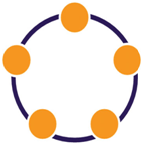
\includegraphics[scale=0.4]{res/archi_cass.png}
\end{wrapfigure}

Cassandra aborde le problème de défaillance (failure) en employant un système distribué peer-to-peer où tous les nœuds sont identiques et les données sont réparties entre tous les nœuds du cluster.
Chaque nœud échange des informations à travers le cluster toutes les secondes.

\vspace{5mm}

Les composants de Cassandra sont les suivants :

\begin{itemize}

\item
\textbf{Gossip} : Permet de découvrir et partager des informations d'emplacement et d'état sur les autres nœuds d'un cluster Cassandra.

\item
\textbf{Partitioner} : Détermine comment distribuer les données entre les nœuds du cluster

\item
\textbf{Stratégie de placement de réplicas} : Détermine les nœuds sur lesquels placer les répliques (La première réplique de données est simplement la première copie)

\item
\textbf{Snitch} : Définit les informations de topologie que la stratégie de réplication utilise pour placer les répliques et les demandes de route de manière efficace.

\item
\textbf{Le fichier cassandra.yaml} : C'est le fichier de configuration principal de Cassandra

\end{itemize}



\subsubsection* {Du point de vue de l'application Client}

\begin{wrapfigure}{r}{-2.5cm}
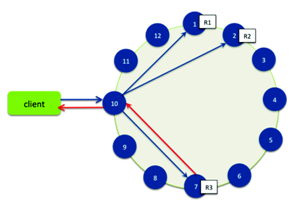
\includegraphics[scale=0.5]{res/cli_cass.png}
\end{wrapfigure}

Tous les nœuds de Cassandra sont égaux. Ainsi, une demande de lecture ou d'écriture peut interroger indifféremment n'importe quel nœud du cluster. Quand un client se connecte à un nœud et demande une opération d'écriture ou de lecture, le nœud courant sert de coordinateur du point de vue du client. Le travail du coordinateur est de se comporter comme un proxy entre le client de l'application et les nœuds qui possèdent la données. C'est lui qui a en charge de déterminer quels nœuds de l'anneau devront recevoir la requête.


\subsubsection* {Caractéristiques}


\begin{itemize}

\item
\textbf{Tolérance aux pannes} : Les données d'un nœud sont automatiquement répliquées vers d'autres nœuds. Ainsi, si un nœud est hors service les données présentes sont disponibles à travers d'autres nœuds.

\item
\textbf{Décentralisé} : dans un cluster tous les nœuds sont égaux. Il n'y pas de notion de maître, ni d'esclave, ni de processus qui aurait à sa charge la gestion.

\item
\textbf{Modèle de données riche} : le modèle de données proposé par Cassandra basé sur la notion de clé/valeur permet de développer de nombreux cas d'utilisation dans le monde du web.

\item
\textbf{Élastique} : la scalabilité est linéaire. Le débit d'écriture et de lecture augmente de façon linéaire lorsqu'un nouveau serveur est ajouté dans le cluster.

\item
\textbf{Haute disponibilité} : possibilité de spécifier le niveau de cohérence concernant la lecture et l'écriture. On parle alors de Tuneable Consistency.

\end{itemize}

\subsubsection* {Modèle de données}

\begin{wrapfigure}{r}{-2.5cm}
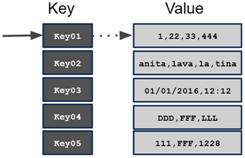
\includegraphics[scale=0.6]{res/model_cass.png}
\end{wrapfigure}

\noindent Apache Cassandra stocke les données dans une suite triée de couples \textbf{clé / valeur}. On classifie ainsi Cassandra comme une base de données NoSQL orientée colonne.

\begin{itemize}

\item
Une \textbf{ligne} est composée d'un ensemble de colonnes et identifiée par une clé

\item
Une \textbf{famille de colonnes} est un regroupement logique de lignes

\item
Un \textbf{Keyspace} est un regroupement de famille de colonnes

\end{itemize}

\begin{center}
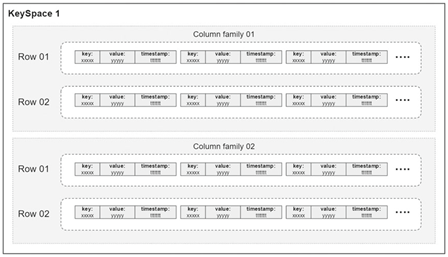
\includegraphics[scale=0.6]{res/model2_cass.png}
\end{center}


\subsubsection* {Connexion avec Spark}

Apache Cassandra utilise l'architecture client/serveur. La connexion entre le client et le serveur peut se faire via :

\begin{itemize}

\item
\textbf{Le CQLs} : c'est un shell pour Cassandra Query Language.

\item
\textbf{Les Drivers} : Il y a des drivers pour Cassandra dans presque tous les langages de programmation modernes (Python, Java, Scala, ...)

\end{itemize}


Pour faire la connexion entre Cassandra et la stack SMACK, et plus précisément avec Spark, nous avons besoin du \textbf{« Spark-Cassandra Connector »}. Ce client est spécial car il est destiné spécifiquement pour Spark, et pas pour un langage spécifié.

\begin{center}
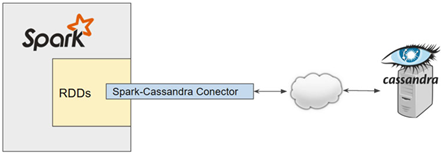
\includegraphics[scale=0.7]{res/spark_cass.png}
\end{center}

\newpage
\subsection {Kafka}

Kafka est une plateforme de streaming distribuée pouvant être utilisée comme un agent de message (message broker). Elle permet à des applications qui échangent des messages en temps réel de les enregistrer et de les distribuer au fur et à mesure avec une latence faible et un débit élevé. De plus, Kafka permet de passer facilement à l'échelle grâce à sa notion de groupe de consommateur détaillé plus bas.


\subsubsection* {Principe de fonctionnement}

Le modèle de fonctionnement de Kafka à haut niveau est simple, les producteurs envoient des messages (de n'importe quel type) à l'un des topic du cluster de Kafka et les consommateurs souscrivent à un ou plusieurs topics :

\begin{center}
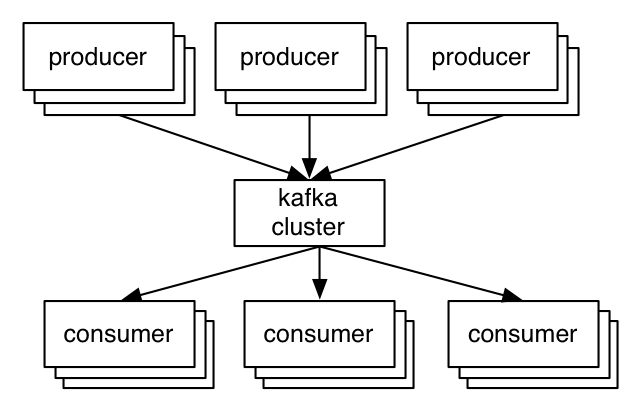
\includegraphics[scale=0.8]{res/producer_consumer.png}
\end{center}

Un topic est en fait un log de tous les messages qui ont étés envoyés par les producteurs. Un topic se décompose en plusieurs partitions afin d'offrir un passage à l'échelle, il n'est donc pas nécessaire qu'une machine soit capable de contenir un topic en entier sur son disque. 


La figure suivante montre un topic composé de 2 partitions :

\begin{center}
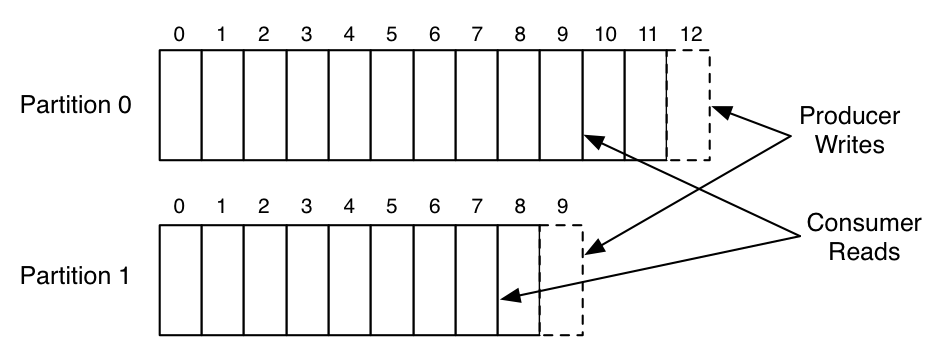
\includegraphics[scale=0.8]{res/topic_kafka.png}
\end{center}

Le producteur écrit chaque message à la suite de l'un des deux topics tandis que le consommateur lit les messages à l'offset qu'il désire (généralement le dernier offset lu + 1).
Les messages sont stockés sur disque et disposent d'une durée de vie configurable au bout de laquelle ils seront supprimés, il est donc possible de les lire dans n'importe quel ordre mais aussi de les relire.
Pour assurer la tolérance aux pannes, chaque partition est écrite sur plusieurs machines.


\subsubsection* {Groupe de consommateur}

Afin de permettre le passage à l'échelle, Kafka propose une notion de groupe de consommateur, cela signifie que chaque message envoyé à un topic sera délivré à un consommateur de chaque groupe souscrivant à ce topic. L'application client utilisant Kafka peut regrouper les consommateurs par groupe à sa guise afin de répartir la charge et d'obtenir la redondance qu'il souhaite. Pour obtenir ce comportement, Kafka donne à chaque consommateur une liste de partitions de taille similaire à traiter qui est modifiée dynamiquement.



\subsubsection* {Garanties et performances}


\begin{itemize}

\item
Un topic répliqué N fois peut supporter N-1 pannes sans perdre de messages.

\item
Kafka nécessite une instance de serveur zookeeper pour fonctionner, celui ci utilise un algorithme proche de paxos et il est donc nécessaire d'avoir une majorité des machines sur lequel zookeeper s'exécute pour assurer le fonctionnement.

\item
Au sein d'une partition, Kafka maintient l'ordre des messages envoyés par un même producteur.

\item
Un consommateur voit les messages dans l'ordre dans lequel ils sont enregistrés sur le topic.

\end{itemize}



% \begin{center}
% % \begin{figure}[ht!]
%     \includegraphics[scale=0.55]{res/sujet_makefiles_premier_Makefile-small_nth4.pdf}
% % \caption{Diagramme des cas d'utilisation}
% % \end{figure}
% \end{center}


\end{document}


